\cotefile{91}
\scanpage{73}
% manuscript line 1
recollement en un morphisme est immédiat.

% manuscript line 2
Par suite, on a défini $W(X)\xrightarrow{\varphi}\unsure{\mathfrak{X}|\mathscr{X}}$.

% manuscript line 3
Je dis que c'est une solution du Pb universel .... i.e\unsure{,|.} que pour tt $T$,
% manuscript line 5
\[
\operatorname{Hom}_S(T,X)\longrightarrow
\operatorname{Hom}_{\underline W(S)}(\underline W(T),\mathfrak{X})
\]
% manuscript line 6
est \uline{bijectif}. Soit \deleted{$u:T\to X$},
% manuscript line 7
\[
\underline W(T)\xrightarrow{\unsure{v|\psi}}\mathfrak{X}
\]
% manuscript line 8
je dis qu'il peut se factoriser de \uline{façon unique} en
% manuscript line 10
\[
\underline W(T)\xrightarrow{\underline W(u)}\underline W(X)
\overset{\varphi}{\unsure{\text{---}|\longrightarrow}}\mathfrak{X}
\]

% manuscript line 11
En effet, \deleted{\unsure{considérons|supposons} \unsure{les|que} \illegible{1}} \deleted{il \unsure{faudr.|faudra} \unsure{que} \unsure{si|l'on ait} on peut factoriser, \unsure{ce} \unsure{soit} $T=\bigcup$} \deleted{$W(u)($} \deleted{\unsure{inversement}} utilisons la condition $(\beta)$\,: $T=\bigcup T_i$, avec $v(\underline W(T_i))\subset\mathfrak{X}_i$. Donc $v|\underline W(T_i))$ est défini par $\unsure{v_i|u_i}:T_i\to X_i$, par factorisation
% manuscript line 18
\[
\underline W(T_i)\xrightarrow{\underline W(u_i)}
 \underline W(X_i)\xrightarrow{\varphi_i}X_i
\]
% manuscript line 19
On vérifie aussitôt que les composés
% manuscript line 20
\[
 T_i\longrightarrow X_i\longrightarrow X
\]
\deleted{$\underline W(T_i)\to\underline W(X_i)\to\underline W(X)$}
% archive sheet number: 72
\scanpage{74}
% manuscript line 1
coïncident dans les $T_i\cap T_j$, donc définissent $T\unsure{\text{---}|\longrightarrow}X$ et ce dernier satisfait aux conditions voulues. D'ailleurs, \deleted{\unsure{toute|t.t|tout}} \unsure{une} solution ne peut, \unsure{à|a} priori, s'obtenir par une construction comme celle qui précède. Introduisant alors les
% manuscript line 7
pour $u,u'$ \unsure{liés|choisis}\,: $(T_i)$, $(T'_j)$, le \unsure{recouvrt|recouvrement} commun $(T_i\cap T'_j)_{i,j\in I\times I'}$), on trouve l'unicité.

% manuscript line 10
\uline{Lemme 3} La condition $\beta$ est automatiquement vérifiée \inserted{(pour tt rec. $\unsure{\mathfrak X|\mathscr X}=\bigcup\mathfrak X_i$ de $\mathfrak X$ par ouverts)} si on a un isomorphisme de foncteurs
% manuscript line 14
\[
|T|\overset{\sim}{\unsure{\longrightarrow|\text{---}}}|\underline W(T)|
\]
% manuscript line 15
en particulier dans les cas $\mathrm{II}'$, \deleted{$\unsure{\mathrm{II}|\mathrm{I}}$}, en particulier $\mathrm{III}$.

% manuscript line 16
C'est trivial.

% manuscript line 17
\uline{Lemme 4} La condition $\alpha$ est automatiquement vérifiée dans les cas $\mathrm{I}',\mathrm{II}^{*}$.

% manuscript line 19
C'est trivial pour $\mathrm{II}^{*}$. Pour $\mathrm{I}'$, petit raisonnement, utilisant que un morphisme fini est \uline{fermé}. (\unsure{Les hyp. inutiles|Sans hyp. noeth.})
% archive sheet number: 73
\scanpage{75}
% manuscript line 1
\uline{Cor} Conclusion \unsure{semblable|valable|satisfaites} dans le cas $\mathrm I$, si $S'$ est propre sur $S$ et si $\underline W^{\unsure{\bullet|\cdot|a}}(\unsure{\mathfrak X|\mathscr X})$ est loc. noeth.

% manuscript line 3
$\overline{\mathrm M}$ raisonnement que pour $\mathrm I'$.

% manuscript line 4
Mettons ensemble les résultats obtenus

% manuscript line 5
\uline{Théorème 1} Dans le cas d'un foncteur de Greenberg \inserted{spécial}, ou d'un foncteur $\underline W_{S'}$ défini
% slanted
\margin{\unsure{dégager|rédiger} \unsure{qqs|par} \unsure{principes}, \unsure{pour}}
% manuscript line 7
par un morphisme $S'\unsure{\longrightarrow|\text{---}}S$ fini, loc. libre, \deleted{\unsure{par}} radiciel, le $W\unsure{^{\wedge}_{\cdot}|?|^{a}}(\mathfrak X)$ existe pour \deleted{tout} préschéma $\mathfrak X$ sur $W(S)$. \deleted{Soit $\mathfrak X=$} $W^{\wedge}$ est de plus un foncteur de \uline{nature locale}

% manuscript line 12
\uline{Théorème 1 bis} \deleted{Dans le cas $\mathrm I$ \unsure{ou} $\mathrm{II}$, $\mathrm I'$,} \inserted{Supposons qu'on soit dans le cas $\mathrm I'$.} \deleted{$\varphi_{S'/S}(\mathfrak X)$} (i) Si $\varphi_{S'/S}(\mathfrak X)$ existe, alors pour tout ouvert $\mathcal U$ de $\mathfrak X$, $\varphi_{S'/S}(\mathcal U)$ existe et $\varphi_{S'/S}(\mathcal U)\unsure{\lhook\joinrel\longrightarrow|\longrightarrow}\varphi_{S'/S}(\mathfrak X)$ est une immersion ouverte.

% manuscript line 18
(ii) Soit $\mathfrak X=\bigcup\mathfrak X_i$, où les $\mathfrak X_i$ sont tels que pour tt $s\in S$, toute \deleted{\unsure{section de}} \inserted{partie finie} de $\mathfrak X_s$ sur $S'_s$ soit contenue dans un $\mathfrak X_i$. Alors si les $\varphi_{S'/S}(\mathfrak X_i)$ existent, $\varphi_{S'/S}(\mathfrak X)$
% archive sheet number: 74
\scanpage{76}
% manuscript line 1
existe et est réunion des $\varphi_{S'/S}(\unsure{\mathfrak X|\mathscr X}_i)$.

% manuscript line 2
Démonstration. Il suffit de prouver (ii), et \unsure{pour ceci|pour cela} de prouver que l'Hyp faite implique la condition de recollement. Or,
% manuscript line 5
si $v:T'\unsure{\longrightarrow|\text{---}}\mathfrak X$ est donné, on introduit les $T'_i=v^{-1}(\mathfrak X_i)$, $\unsure{\longrightarrow|\text{---}}$ et les $T_i=\complement\,\varphi_T(T'-T'_i)$, qui sont des ouverts de $T$, on est ramené à prouver que $T=\bigcup T_{\unsure{i|ij}}$.
\diagram{\begin{tikzcd}[ampersand replacement=\&,column sep=small,row sep=small]
 \& \mathfrak X\arrow[d]\\
 S \& S'\arrow[l,"\varphi"']\\
 T\arrow[u] \& T'\arrow[u]\arrow[l,"\unsure{\varphi_T|\varphi'_T}"]\arrow[uu,dashed,bend right=36,"v"']\\
 \&\mathfrak X_s\\
 k(s)\& S'_s\\
 k(t)\& T'_t
\end{tikzcd}}
% manuscript line 9
\deleted{et pour ceci, il.} Or $t\in T_i$ signifie que la restriction à $T'_t$ de $\varphi$ applique $T'_t$ dans $\mathfrak X_i$\,: donc une section de $(\mathfrak X_s/S'_s)_{/k(s)}$ définie sur l'extension $k(t)$ de $k(s)$, doit être contenue dans un des $\mathfrak X_i$.
% manuscript line 14
\deleted{Or si on décompose $\mathfrak X_s$ \inserted{en des $\mathfrak X_s^\alpha$} suivant les compos. connexes \inserted{$S_s^{\prime\alpha}$} \unsure{des} $S_s^{\prime\alpha}$, \unsure{cela revient à} \unsure{ce} que dès que a une section de $\mathfrak X_i^\alpha$ sur \illegible{1}}

% manuscript line 18
% slanted
\margin{Soit $n(s)$ le \deleted{\unsure{n. des}} \deleted{\unsure{points}} \unsure{rang} géom. des fibres de $S'/S$}
\uline{Corollaire 1} Si Toute partie \deleted{\unsure{aff}} finie \inserted{ayant $\leq n(s)$ \unsure{élémts}} d'un $\mathfrak X_s$ est contenue dans un ouvert affine de $\mathfrak X$, \deleted{alors} [en particulier si \deleted{les $\mathfrak X_s$} $\mathfrak X/S$ \deleted{les} sont quasi-projectifs] alors $\varphi_{S'/S}(\mathfrak X)$ existe, et est
% archive sheet number: 75
\scanpage{77}
% manuscript line 1
réunion des $\varphi_{S'/S}(\mathcal U)$, où $U$ parcourt les ouverts affines de $\unsure{\mathfrak X|\mathscr X}$.

% manuscript line 3
\uline{Corollaire 2} Supposons \deleted{\uline{de plus}} \inserted{que tte partie finie de $\mathfrak X$ soit contenue dans un ouvert affine, et} $\mathfrak X$ de type fini \inserted{sur $S'$,} et $S$ loc. noeth. Alors $\varphi_{S'/S}(\mathfrak X)$ est de type fini sur $S$.

% manuscript line 6
La question étant locale \inserted{sur $S$}, on peut supposer $S$ affine. Tout résulte du

% manuscript line 8
\uline{Lemme} Soit $S$ noethérien, $\mathfrak X$ de type fini sur $S$, $n$ un entier. \inserted{\deleted{\unsure{les|Soit}} $(\mathfrak X_i)_{i\in I}$ famille d'ouverts,} On suppose que tte partie \deleted{finie} $E$ de $\mathfrak X$ telle que $\operatorname{card}(E)\leq n$ est contenue dans un ouvert \deleted{affine \unsure{de}} $\mathfrak X_i$. Alors il existe une \unsure{ss-famille|sous-famille} finie de $(\mathfrak X_i)_{i\in I}$ ayant la $=$ propriété.

% manuscript line 15
En effet, l'hyp. signifie que
% manuscript line 16
\[
\bigcup_{i\in I}
\underbrace{\mathfrak X_i\times_S\text{---}\times_S\mathfrak X_i}_{n\text{ facteurs}}
=
\underbrace{\mathfrak X\times_S\text{---}\times_S\mathfrak X}_{\unsure{n|\text{---}}\text{ facteurs}}.
\]
% manuscript line 17
On applique le fait que $\mathfrak X\times_S\text{---}\times_S\mathfrak X$ est \inserted{un espace} noethérien.

% manuscript line 19
$\unsure{\mathbb Z|2}$. Le foncteur $\underline W^{\unsure{\underline a|\wedge|a}}$ n'est pas local en tous les \unsure{cas}. Cas où il n'existe pas \unsure{même}
% archive sheet number: 76
\scanpage{78}
% manuscript line 1
4) \uline{Applications aux immersions, etc}

% manuscript line 2
\uline{Proposition} Supposons que $\underline W$ soit \deleted{\uline{\unsure{spécial}} \unsure{et} $\mathrm I'$ \unsure{ou} $\mathrm{II}$} \inserted{$\mathrm I'$, ou Greenberg spécial}.

% manuscript line 3
Soit $f:\unsure{\mathfrak X|\mathscr X}\longrightarrow\unsure{\mathfrak Y|\mathscr Y}$ un morphisme d'immersion \deleted{\unsure{resp.}} fermée \inserted{\deleted{(resp. de type fini)}}. Supposons \deleted{\unsure{de|dans de}} \deleted{\unsure{que}} dans le cas $\mathrm I'$ que \deleted{$\underline W^{\unsure{a|\bullet}}(\mathfrak Y)$ existe et est réunion des $\underline W^{\bullet}(\mathcal U)$, $\mathcal U$ affines dans $\mathfrak Y$.} tte partie finie d'un $\mathfrak Y_s$ est contenue dans un ouvert affine de $\mathfrak Y$. \deleted{Alors $\underline W^{a}(\mathfrak X)$ existe,} et $\underline W^{\bullet}(f)$ \inserted{(existe et)} est une immersion fermée.

% manuscript line 11
En effet, on est ramené au cas affine, où \unsure{cel|cela|celà} a été vu.

% manuscript line 13
\uline{Corollaire} \inserted{Dans les conditions précédentes sur $W$} Si $\mathfrak Y$ est quasi-projectif sur $S^{*}$, et si $f:\mathfrak X\to\mathfrak Y$ est une immersion, alors $\underline W^\wedge(f)$ est une immersion.

% manuscript line 16
En effet, $f$ se factorise en
% manuscript line 17
\[
\mathfrak X\overset{f'}{\unsure{\text{---}|\longrightarrow}}
\mathfrak X'\overset{f''}{\text{---}}\mathfrak Y
\]
% manuscript line 18
\deleted{\unsure{imm.|avec}} $f'$ une imm. fermée et $f''$ imm. ouverte. $\mathfrak X'$ sera \unsure{aussi} quasi projectif, on
% archive sheet number: 77
\scanpage{79}
% manuscript line 1
applique la prop à $f'$, et on \unsure{applique ens.|appliquera|applique} \unsure{le $=$|$=$} à $f''$.

% manuscript line 2
\deleted{Prop} \uline{Corollaire 2} Sous les conditions de la prop. pour $\underline W$, \deleted{$\unsure{\mathfrak X|\mathscr X}$ \unsure{Si}} supposons que \deleted{$\mathfrak X$ et $\unsure{\mathfrak Y|\mathscr Y}$} tte partie finie de $\mathfrak X$ soit contenue dans un ouvert affine. Alors si $f:\mathfrak X\to\mathfrak Y$ est séparé, alors il en est de même de $\underline W^{\unsure{\bullet|a}}(f)$ [sous réserve que $\underline W^\wedge(\mathfrak Y)$ existe dans le cas $\mathrm I'$].

% manuscript line 9
On applique la prop à $\mathfrak X\unsure{\text{---}|\longrightarrow}\mathfrak X\times_{\mathfrak Y}\mathfrak X$.

% manuscript line 10
\uline{Proposition} $W$, \deleted{$\unsure{\mathcal U|\mathfrak X}$} $\mathfrak Y$ comme dans la prop. précédente. Soit $f:\mathfrak X\to\mathfrak Y$, on suppose \deleted{\unsure{déjà|affine}} \inserted{dans le cas $\mathrm I'$} que pour tout ouvert affine \inserted{$U$} de $\mathfrak Y$, \inserted{tte partie finie de} $f^{-1}(U)$ est \deleted{réunion} contenue dans un ouvert affine (p. ex. $f$ quasi-projectif). On suppose de plus $\mathfrak Y$ loc. noeth et \deleted{$\mathfrak X$.} $f$ de type fini. \inserted{\deleted{(resp. affine)}} Alors $\underline W^{a}(f)$ est de type \unsure{finie|fini} \deleted{(resp. affine)}.
% slanted
\margin{\unsure{rédiger cela|restreig. à cela}. \unsure{Donner|Dans} le cas ``Greenberg spécial''\unsure{;|,} l'autre est \unsure{une} variante \unsure{contenue|continue|remplacée} dans le premier \unsure{(car} projectif $\Rightarrow$ quasi-projectif\unsure{)}}.
% archive sheet number: 78
\scanpage{80}
% manuscript line 1
\uline{Proposition} Comme dessus, pour morphismes \uline{affines}.
% archive sheet number: 79
\scanpage{81}
% manuscript line 1
\deleted{\uline{\unsure{Notion|Notions} \unsure{d'espace|d'espaces}} \uline{\unsure{non} \illegible{1}}}

% manuscript line 3
\uline{\unsure{Schèmas|Schémas} localement} \uline{compacts}
% archive sheet number: 80
\scanpage{82}
% manuscript line 1
$Z$ constructible dans $X$ quasi compact, \inserted{dont} tt pt a un syst. fond. de voisinages rétrocompacts dans $X$.
% manuscript line 2
\deleted{$Z$ loc constructible}
% manuscript line 3
\[
\left\{\begin{aligned}
&Z\text{ quasi cpct et}\\
&\forall x\in Z,\ \exists\text{ un voisinage }U_x\text{ de }x\text{ dans }X,\text{ tel que }Z\cap U_x\text{ constr. dans }U_x\\
&\text{(alors tt ouvert }U'\subset U,\ U'\ni x,\text{ a la }=\text{ propriété)}.
\end{aligned}\right.
\]
% manuscript line 6
Nécessité évidente [car $Z$ rétrocompact dans $X$, \deleted{\unsure{donc}} quasi cpct et on peut prendre $U=X$

% manuscript line 8
Suffisance. $Z$ est recouvert par un nb fini des $U_x$, \unsure{soient|soit} $U_i$. les $U_i\cap Z$ sont constructibles dans $U_i$, donc dans $X$, donc $Z=\bigcup Z_i$ est constr.

% manuscript line 11
\uline{Corollaire} Supposons $Z$ loc. fermé. Alors $Z$ \deleted{loc.} constructible ssi $Z$ est \uline{quasi compact}, et tt pt $x\in Z$ a un voisinage ouvert $U$ dans $X$ tel que $Z\cap U$ \deleted{soit fermé} \deleted{\unsure{comm|et}} \uline{constructible} dans $U$, i.e. $U-Z\cap U$ rétro-\deleted{\unsure{cp.}}ct dans $U$ [i.e. $U-Z\cap U$ quasi-compact, si on \inserted{prend $U$ quasi-cpct, et si on} suppose que dans $X$, l'intersection de deux ouverts quasi cpcts est quasi cpcte).

% manuscript line 18
\uline{Exemple} Si $X$ est un préschéma quasi-séparé quasi-compact (p. ex. un schéma quasi-compact, tel un schéma affine) \deleted{\unsure{Alors}} $Z$ loc. fermé dans $X$, alors $Z$ constructible $\Longleftrightarrow$ $Z$ quasi cpct, \uuline{et} tt $x\in Z$ a un voisinage ouvert affine $U$ tel que $Z\cap U$ soit défini par un \uline{nb fini} d'\uline{équations}
% archive sheet number: 81

% Reverse-face typescript shows through here. See scan 83.
\scanpage{83}
% manuscript line 1
\mspage{- 122 -}n\textsuperscript{o} 316

% manuscript line 2
$V_{(L)}$ est muni canoniquement d'une structure d'espace vectoriel topologique métrisable et complet (\uline{Esp}. \uline{vect}. \uline{top}. chap.I, § 2, n\textsuperscript{o}3, th.2).
% manuscript line 4
Soit $(x_p)_{p\handwritten{\in}z}$ une famille d'éléments de $V$ tels que $x_p=0$ pour $p$ inférieur à un certain entier rationnel. Alors la série $\mathop{\handwritten{\sum}}\nolimits_{\handwritten{-\infty}}^{\handwritten{+\infty}}x_p T^p$ converge dans $V_{(L)}$, et tout élément de $V_{(L)}$ se met sous cette forme de manière unique. (Prendre une base dans $V$).

% manuscript line 8
b) L'espace vectoriel $\handwritten{\unsure{\mathscr L|\mathcal L}}_L(V_{(L)})=(\handwritten{\mathscr L}_K(V))_{(L)}$ est muni canoniquement d'une structure d'espace vectoriel topologique métrisable et complet. Tout endomorphisme de $V_{(L)}$ se met d'une manière unique sous la forme $\mathop{\handwritten{\sum}}\nolimits_{\handwritten{-\infty}}^{\handwritten{+\infty}}u_pT^p$, où $u_p\handwritten{\in}\handwritten{\mathscr L}_K(V)$, et où les $u_p$ sont nuls pour $p$ inférieur à un certain entier rationnel.

% manuscript line 13
c) Si $K$ est de caractéristique $0$, et si $u\handwritten{\in}\handwritten{\mathscr L}_K(V)$, on pose $e^{Tu}={}=1+\frac{1}{1!}\,u\,T+\frac{1}{2!}\,u^2\,T^2+\ldots\handwritten{\in}\handwritten{\mathscr L}_L(V_{(L)})$. Si $x\handwritten{\in}V$ est tel que $u\,x=0$, on a $e^{Tu}.x=x$.

% manuscript line 16
d) Si $W$ est un autre espace vectoriel de dimension finie sur $K$, et si $v\handwritten{\in}\handwritten{\mathscr L}_K(W)$, on a $e^{T(u\handwritten{\otimes}1+1\handwritten{\otimes}v)}=e^{Tu}\handwritten{\otimes}e^{Tv}$.

% manuscript line 18
e) Déduire de c) et d) que, si $V$ est muni d'une structure d'algèbre
% archive sheet number: 82
\scanpage{84}
% manuscript line 1
\figure{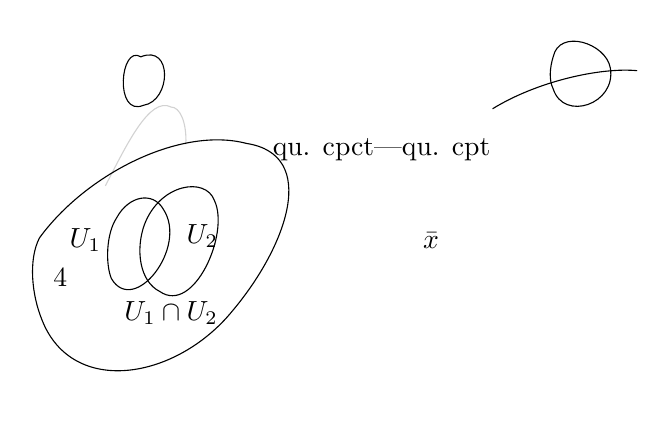
\begin{tikzpicture}[x=.011cm,y=-.011cm]
\draw (42,32) .. controls (18,17) and (11,102) .. (45,88)
 .. controls (77,83) and (79,17) .. (42,32);
\draw[gray!35] (1,181) .. controls (25,135) and (52,77) .. (77,90)
 .. controls (87,90) and (95,107) .. (94,133);
\draw (-75,241) .. controls (-21,167) and (88,112) .. (164,132)
 .. controls (248,145) and (211,250) .. (148,325)
 .. controls (83,405) and (-37,425) .. (-72,336)
 .. controls (-84,307) and (-88,266) .. (-75,241);
\draw (14,218) .. controls (28,192) and (56,187) .. (68,208)
 .. controls (97,252) and (34,332) .. (8,288)
 .. controls (1,271) and (2,236) .. (14,218);
\draw (46,226) .. controls (64,178) and (117,170) .. (127,198)
 .. controls (145,236) and (103,330) .. (64,303)
 .. controls (40,291) and (36,254) .. (46,226);
\node at (-22,244) {$U_1$}; \node at (113,239) {$U_2$};
\node at (77,328) {$U_1\cap U_2$}; \node at (-51,287) {$4$};
\node[anchor=west] at (183,139) {\unsure{qu. cpct|qu. cpt}};
\draw (518,32) .. controls (525,-1) and (579,16) .. (584,45)
 .. controls (591,87) and (530,107) .. (518,69) .. controls (513,59) and (514,45) .. (518,32);
\draw (448,92) .. controls (500,60) and (573,44) .. (615,48);
\node at (377,244) {$\bar x$};
\end{tikzpicture}}

% manuscript line 2
\margin{Supposons que tt pt de $X$ a un syst. fond. de voisinages ouverts, rétrocompacts dans $X$. [Alors tte partie ouverte quasi-cpte de $X$ est rétrocompacte]}
\par\noindent\rule{.94\linewidth}{.3pt}

% manuscript line 5
\margin{$\unsure{E|F|Z}$\par $U$}
Soit $\deleted{\unsure{F|E}}T$ une partie fermée irréductible de $X$.

% manuscript line 6
Conditions équivalentes

% manuscript line 7
(i) Il existe une partie $Z$, ouverte non vide dans $T$, telle que $Z$ soit constructible \unsure{dans} $X$

% manuscript line 9
(ii) Il existe un ouvert \inserted{quasi-compact} $U$ de $X$, tel que $U\cap T\ne\varnothing$, et $U-U\cap T$ soit quasi cpct.
% archive sheet number: 83
% Faint type visible in reverse is on the other face of the paper.
\scanpage{85}
% manuscript line 1
\[
\mathop{\handwritten{\sum}}\nolimits_{j=0}
(x_1\,T_1+\ldots+x_{k-1}\,T_{k-1})^j\,x_k\,T_k\,
(x_1 T_1+\ldots+x_{k-1}\,T_{k-1})^{k-j-1}
\]

% manuscript line 2
Etant donnés deux éléments $x,y$ de $L$, on définit $g_{i,k-1}(x,y)$ comme le coefficient de $T_1^i\,T_2^{k-i}$ dans $(x\,T_1+y\,T_2)^k$. Montrer que l'on a
% manuscript line 4
\[
i!\,(k-i)!\,g_{i,k-i}(x,y)=f_k(t_1,\ldots,t_k)
\]
% manuscript line 5
avec $t_h=x$ pour $h\handwritten{\leqslant}i$ et $t_h=y$ pour $h\handwritten{\geqslant}i+1$.

% manuscript line 6
b) Lorsque $L$ est considérée comme algèbre de Lie sur $K$, on a , dans $\handwritten{\unsure{\mathscr L|\mathcal L}}_K(L)$\,:
% manuscript line 7
\[
(\mathrm{ad}\,x)^n=\mathop{\handwritten{\sum}}\nolimits_{i=0}^{n}
(-1)^{n-i}\binom{n}{i}\,L_x^i\,R_x^{n-i}.
\]
% manuscript line 8
En déduire que, si $K$ est de caractéristique $p$ ($p$ premier), on a\,:
% manuscript line 9
\begingroup
\makeatletter
\tagsleft@true
\makeatother
\[
(\mathrm{ad}\,x)^p.y=(\mathrm{ad}\,x^p).y
\tag*{(1)}
\]
% manuscript line 10
\[
(\mathrm{ad}\,x)^{p-1}.y=\mathop{\handwritten{\sum}}\nolimits_{i=0}^{p-1}x^i\,y\,x^{p-1-i}
\tag*{(2)}
\]
\endgroup

% manuscript line 11
Déduire de (2) que\,:
% manuscript line 12
\[
f_{p-1}(\mathrm{ad}\,x_1,\ldots,\mathrm{ad}\,x_{p-1}).y=f_p(x_1,\ldots,x_{p-1},y)
\]
% manuscript line 13
et\,:
% manuscript line 14
\[
g_{i,p-1-i}(\mathrm{ad}\,x,\mathrm{ad}\,y).y=(p-i)\,g_{i,p-i}(x,y).
\]
% archive sheet number: 84
